% Programacao Concorrente (ICP-361) (IC/UFRJ)
% Abril de 2024
% Prof.: Silvana Rossetto
% Trabalho: Implementação de uma aplicação concorrente

\documentclass[14]{article}
\usepackage{color,graphicx}
\usepackage{../sbc-template}
\usepackage{listings}
\usepackage{hyperref}
\hypersetup{
    colorlinks=true,
    linkcolor=blue,
    filecolor=magenta,      
    urlcolor=blue,
    pdfpagemode=FullScreen,
}

\renewcommand{\refname}{Bibliografia}
\begin{document}

\title{{\em Jogo Paralelo da Vida}

{\em \normalsize Gabriel Duarte Soares - 122078892 \and  Henrique Lima Cardoso - 122078397}
\author{ {\Large Relatório Parcial} Programação Concorrente (ICP-361) --- 2024/2}
\address{} 
\date{}}

\maketitle

\tableofcontents

\section{Descrição do Problema Geral}  
O projeto consiste na simulação de autômatos celulares, um 
\href{https://en.wikipedia.org/wiki/Zero-player_game}{Jogo de Zero Jogadores}, 
onde o espaço é dividido em células que mudam de estado ao longo do tempo, seguindo um conjunto de regras específicas.  
Especificamente, simulamos o 
\href{https://en.wikipedia.org/wiki/Conway's_Game_of_Life}{Game of Life} criado por 
\href{https://en.wikipedia.org/wiki/John_Horton_Conway}{John Conway}.  
Nesse jogo, cada célula pode estar "viva" ou "morta", e seu estado em cada iteração é determinado pelas condições das células vizinhas.  

As regras padrão do \textit{Game of Life} são:  
\begin{itemize}
    \item Uma célula viva com menos de dois vizinhos vivos morre (\textit{subpopulação}).  
    \item Uma célula viva com dois ou três vizinhos vivos continua viva (\textit{sobrevivência}).  
    \item Uma célula viva com mais de três vizinhos vivos morre (\textit{superpopulação}).  
    \item Uma célula morta com exatamente três vizinhos vivos torna-se viva (\textit{reprodução}).  
\end{itemize}  

Implementamos o jogo tanto de forma sequencial quanto concorrente, utilizando as linguagens \textbf{C} e \textbf{Go}:  
\begin{itemize}
    \item \textbf{Em C}, utilizamos mecanismos de concorrência como \textit{threads}, e implementamos \textit{canais} e \textit{waitGroups} para coordenar a execução das simulações paralelas.  
    \item \textbf{Em Go}, exploramos dois modelos de paralelismo:  
    \begin{itemize}
        \item Execuções concorrentes com chamadas a funções via \texttt{go func}.  
        \item Uso de \texttt{goroutines} duradouras, que recebiam mensagens para atualizar o estado do sistema.  
    \end{itemize}
\end{itemize}  

A configuração inicial do grid foi gerada aleatoriamente, e o programa foi testado com diferentes entradas, todas definidas pelo usuário:  
\begin{itemize}
    \item \textbf{Dimensões do grid}: por exemplo, 256x256 ou 1024x1024.  
    \item \textbf{Número de iterações}: por exemplo, 512 ou 1024
    \item \textbf{Número de threads}: por exemplo, 8 ou 16
\end{itemize}

%-----------------------------------------------------------------------
\section{Projeto da solução concorrente}

Ao implementar uma solução concorrente para a simulação de autômatos celulares, a tarefa principal — a atualização do grid ao longo do tempo — pode ser dividida entre diferentes threads ou rotinas paralelas, acelerando significativamente o programa.  

Inicialmente, dividimos o espaço da maneira mais simples possível, atribuindo blocos para cada thread de forma a isolar o espaço de atuação de cada uma delas. Nesse sentido, o programa é \href{https://en.wikipedia.org/wiki/Embarrassingly_parallel}{embaraçosamente paralelo}.  

Para paralelizar o código, implementamos a atualização do grid utilizando duas matrizes: uma para leitura e outra para escrita. A cada iteração, as threads liam os estados passados das células na matriz de leitura e calculavam os novos estados, que eram escritos na matriz de escrita. Após todas as threads concluírem suas operações, as matrizes eram trocadas, reduzindo o número de alocações de memória, já que sempre reaproveitávamos as mesmas duas áreas contíguas de memória.  

A implementação foi feita tanto em \textbf{Go} quanto em \textbf{C}, utilizando estruturas similares às "barreiras" discutidas em aula:  
\subsection{Em Go}
    Testamos duas abordagens:  
    \begin{itemize}  
        \item Chamadas a novas funções paralelas (\texttt{go func}) para atualizar partes do grid.  
        \item \texttt{Goroutines} permanentes que aguardavam mensagens para atualizar o grid.  
    \end{itemize}  
    Ambas as soluções realizavam balanceamento de carga automaticamente, pois as goroutines processavam tarefas assim que estavam disponíveis. Ao testar diferentes formas de dividir os blocos entre as goroutines, a melhor abordagem foi dividir o grid por linhas, simplificando o código e garantindo localidade nos acessos à memória, obtendo assim uma aceleração maior.  
\subsection{Em C}

Adaptamos as ideias da implementação em Go, criando estruturas similares às utilizadas nessa linguagem:  
    \begin{itemize}  
        \item \textit{Canais} para implementar o sistema de mensagens entre as threads.  
        \item \textit{WaitGroups} para garantir a sincronização entre as threads e a main thread ao final de cada iteração.  
        \item Um \textit{pool} de threads, que recebia mensagens da main thread para atualizar as partes do grid atribuídas.  
    \end{itemize}  
    Implementamos o \textit{pool} de threads para minimizar o overhead associado à criação de novas threads a cada iteração, reaproveitando threads já alocadas para melhorar o desempenho.

    Todas as implementações podem ser acessadas no repositório do projeto: \url{https://github.com/dsgab/game-of-life}.  


%-----------------------------------------------------------------------
\section{Teste de Corretude}  

Para garantir a corretude do programa, implementamos versões sequenciais do \textit{Game of Life}, tanto em \textbf{C} quanto em \textbf{Go}, utilizando a mesma abordagem com duas matrizes (uma para leitura e outra para escrita).  
O teste de corretude consistiu em comparar, após cada iteração, o resultado da versão concorrente com o da versão sequencial. Essa comparação era simples, verificando se ambas as matrizes (da versão concorrente e da sequencial) eram idênticas ao final de cada iteração.  

Após muitos erros corrigidos — principalmente relacionados aos mecanismos concorrentes na implementação em \textbf{C} — conseguimos fazer com que ambas as versões agissem de maneira consistente em todas as entradas testadas. Após validar a corretude, removemos os testes de comparação do fluxo principal do programa, mas a função utilizada para realizar essa validação permanece no código como uma utilidade não utilizada.  

Durante o processo de depuração, utilizamos o \textbf{Valgrind}, especialmente uma ferramenta chamada \textit{Helgrind}, que nos ajudou a identificar e corrigir erros de \textit{data races}. Esses erros estavam causando inconsistências, especialmente em cenários com um grande número de iterações ou grids de tamanho maior.  
Um caso notável foi um problema em nossa implementação de um modelo produtor-consumidor, que estava ligeiramente errado. Após identificar e corrigir o erro com a ajuda do \textit{Helgrind}, conseguimos resolver as inconsistências no comportamento do programa.  

{
    \small
    \begin{lstlisting}[breaklines]
        ==33655== Possible data race during write of size 8 at 0x4A8B408 by thread #1
        ==33655== Locks held: none
        ==33655==    at 0x109C50: insert (in /home/hq/gits/game-of-life/c-life/bin/main)
        ==33655==    by 0x10A046: iterate_concurrently (in /home/hq/gits/game-of-life/c-life/bin/main)
        ==33655==    by 0x109577: main (in /home/hq/gits/game-of-life/c-life/bin/main)
        ==33655== 
        ==33655== This conflicts with a previous read of size 8 by thread #16
        ==33655== Locks held: none
        ==33655==    at 0x109CB0: take_out (in /home/hq/gits/game-of-life/c-life/bin/main)
        ==33655==    by 0x109ECB: thread_work (in /home/hq/gits/game-of-life/c-life/bin/main)
        ==33655==    by 0x4854B7A: ??? (in /usr/libexec/valgrind/vgpreload_helgrind-amd64-linux.so)
        ==33655==    by 0x4911A93: start_thread (pthread_create.c:447)
        ==33655==    by 0x499EA33: clone (clone.S:100)
        ==33655==  Address 0x4a8b408 is 104 bytes inside a block of size 320 alloc'd
        ==33655==    at 0x48488A8: malloc (in /usr/libexec/valgrind/vgpreload_helgrind-amd64-linux.so)
        ==33655==    by 0x109B68: create_ch (in /home/hq/gits/game-of-life/c-life/bin/main)
        ==33655==    by 0x109F16: create_pool (in /home/hq/gits/game-of-life/c-life/bin/main)
        ==33655==    by 0x109561: main (in /home/hq/gits/game-of-life/c-life/bin/main)
        ==33655==  Block was alloc'd by thread #1    
    \end{lstlisting}  
}
    
    
    

% Descrever como o programa será testado:

% Para avaliar o desempenho, os testes devem medir o tempo de execução da solução concorrente para diferentes tamanhos de grids 
% e números de threads. Espera-se que o tempo de execução diminua  significativamente com o aumento do número de threads.

% Como o output do programa é uma sequência de tabelas - ou estado do universo. Quando testarmos a corretude do programa,
% teremos que comparar a solução paralela com a solução sequencial para cada frame. Isso será fácil de fazer, pois não envolve
% a parte gráfica - da visualização do programa.

% Para testar o desempenho, olharemos para grids com dimensões distintas (pequeno até enorme).
% Podemos querer saber também a interferência na densidade de células vivas inicialmente.

% Espera-se que o programa tenha quase 100\% de eficiência! Isto é: o speedup é linear em relação ao número de threads.
% Mas em grids pequenos, a sobrecarga de comunicação pode limitar os ganhos, diminuindo a eficiência.

% Se tivermos a oportunidade de implementar técnicas mais avançadas para a atualização do autômato,
% será divertido também observar qual é o impacto da paralelização.



\section{ Avaliação de desempenho}

Para realizar a comparação entre as implementações em Go e C do Jogo da Vida concorrente, fizemos algumas alterações nos programas para facilitar a medição do tempo de execução. Especificamente, ajustamos os outputs para que fossem apenas números em ponto flutuante, representando os tempos de execução em segundos. No caso do programa em Go, foram impressos dois valores: o tempo de execução para a implementação com \texttt{go func} e para a implementação com \texttt{pooling}.

\subsection{Automatização de Execuções e Coleta de Resultados}

Desenvolvemos um programa Python (\texttt{cria\_csv.py}) para realizar testes automatizados em ambas as implementações, considerando as seguintes combinações de entradas:
\begin{itemize}
    \item Tamanhos do lado do tabuleiro: \{32, 128, 512, 1024\}.
    \item Números de iterações: \{256, 512, 1024\}.
    \item Números de threads: \{1, 2, 4, 8, 16\}.
\end{itemize}

Cada combinação de entrada foi executada 5 vezes, calculando-se a média dos tempos medidos. Os resultados foram armazenados em dois arquivos CSV:
\begin{itemize}
    \item \texttt{c\_values.csv}: contendo os resultados da implementação em C.
    \item \texttt{go\_values.csv}: contendo os resultados da implementação em Go (ambas as abordagens concorrentes).
\end{itemize}

\subsection{Visualização de Resultados}

Para analisar os dados coletados, criamos um notebook Jupyter \texttt{le\_csv.ipynb}, que permitiu a visualização de maneira clara e comparativa. Para cada combinação de tamanho do lado do tabuleiro e número de iterações, os seguintes gráficos foram gerados:

\begin{itemize}
    \item \textbf{Tempo de execução em relação ao número de threads}: mostrando a performance de cada abordagem concorrente (C, Go com \texttt{go func} e Go com \texttt{pooling}).
    \item \textbf{Tempo de execução em relação ao número de threads em escala logarítmica}: para facilitar a comparação das tendências de desempenho.
    \item \textbf{Aceleração em relação ao número de threads}: mostrando o ganho de desempenho relativo de cada implementação em comparação à execução sequencial (1 thread).
    \item \item \textbf{Eficiência em relação ao número de threads}: avaliando a relação entre aceleração e número de threads utilizadas e o speed-up atingido.
\end{itemize}

Os gráficos permitiram identificar diferenças importantes entre as abordagens, como a eficiência do gerenciamento de threads em Go e C e o impacto do balanceamento de carga (ou falta dele) em cada implementação. A análise detalhada dos resultados será discutida na próxima seção.

\begin{figure}[!h]
    \begin{center}
    \caption{Gráfico de Eficiência obtido (outros podem ser vistos no Notebook)}
    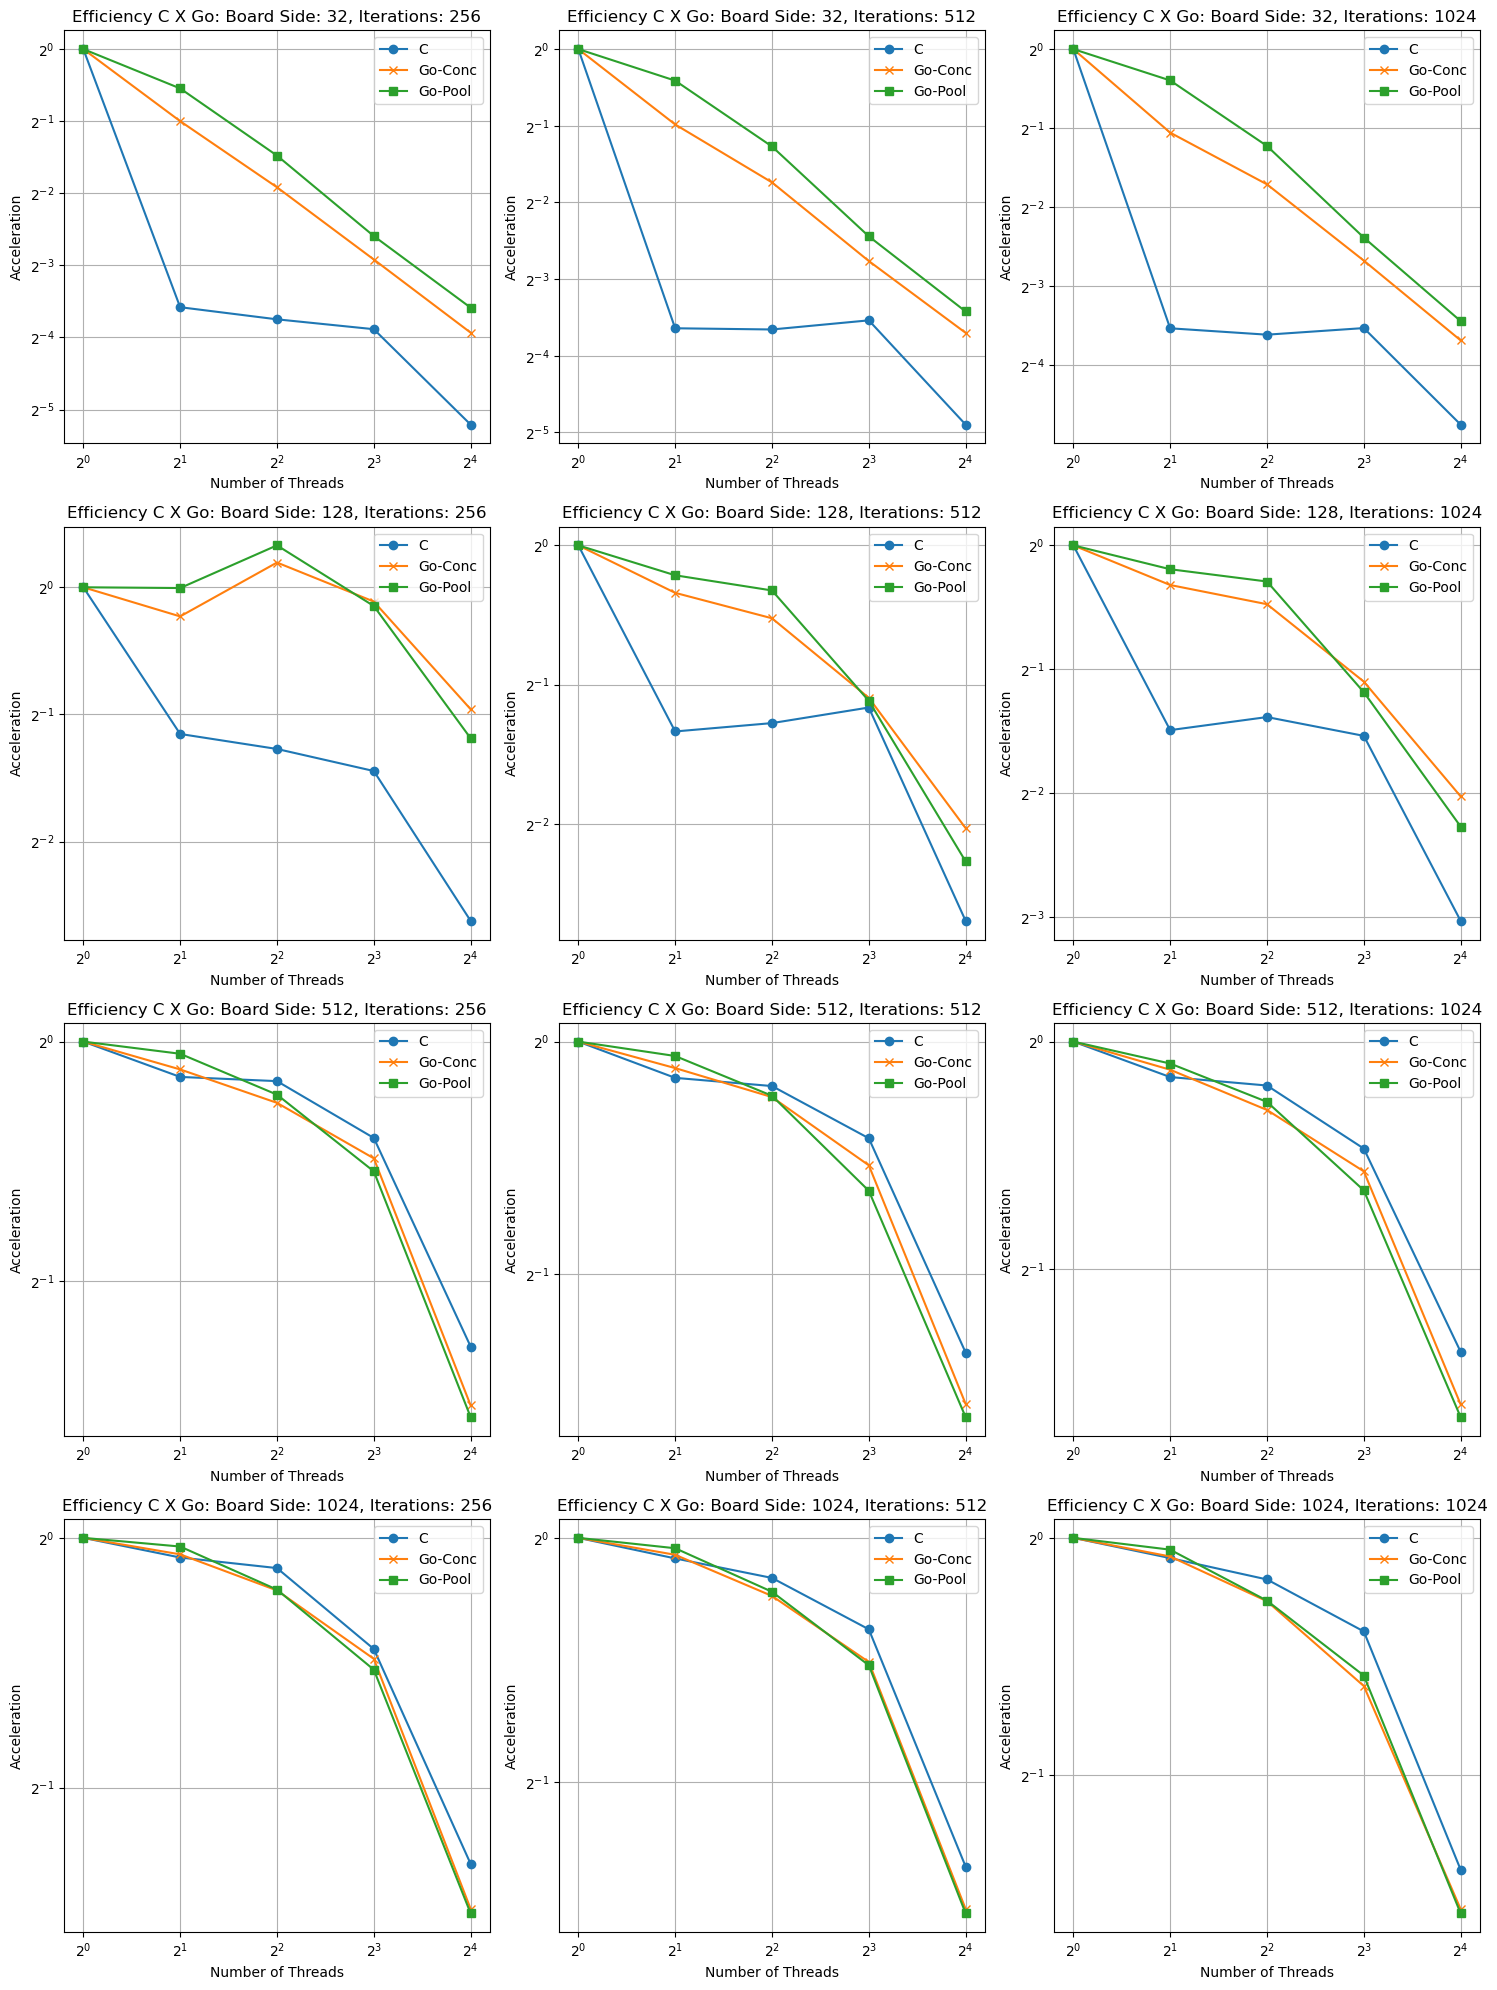
\includegraphics[width=\textwidth]{grafico_eficiencia.png}
    \end{center}
\end{figure}

\section{ Discussão }

Os resultados obtidos nos testes confirmaram algumas expectativas teóricas e revelaram observações interessantes sobre o desempenho relativo das implementações em Go e C, tanto sequenciais quanto concorrentes.

\subsection{Desempenho Sequencial}

Nos testes com as versões sequenciais dos programas, observamos que a implementação em C era consistentemente mais rápida do que a em Go, geralmente apresentando um desempenho cerca de duas vezes melhor. Esse resultado era esperado, já que C é uma linguagem de mais baixo nível, permitindo otimizações mais diretas no acesso à memória e no gerenciamento de recursos. Entretanto, esse cenário se inverteu para inputs pequenos, onde Go demonstrou vantagens devido à leveza inerente de sua abordagem para tarefas concorrentes.

\subsection{Speedup Superlinear}

Um comportamento notável foi a ocorrência de \textbf{speedup superlinear} em algumas configurações específicas no Go, particularmente para grids de tamanho \(128 \times 128\) e 256 iterações. Esse fenômeno pode ser explicado pela melhora na localidade de memória e pela redução de \textit{cache misses}, dado que o particionamento das tarefas entre múltiplas threads possivelmente maximizou o uso de memória local para essas configurações.

\subsection{Pooling versus \texttt{go func} em Go}

Ao comparar as duas estratégias de concorrência em Go – uma com threads vivas esperando por mensagens (\textit{pooling}) e outra com chamadas a \texttt{go func} a cada iteração –, os resultados foram bastante similares. Para inputs pequenos, a versão com \textit{pooling} apresentou desempenho ligeiramente superior, mas o ganho foi negligente. Na prática, o uso de \texttt{go func} demonstrou ser consideravelmente mais simples do ponto de vista da lógica do código. Isso destaca a eficácia do \textit{scheduler} nativo de Go, que gerencia automaticamente o balanceamento e a reutilização de goroutines de forma muito eficiente. Essa observação reforça uma lição importante para o futuro: soluções mais simples frequentemente são mais vantajosas.

\subsection{Desempenho em C com Pooling de Threads}

Na implementação em C, usamos um sistema de \textit{pooling} de threads que simulava o comportamento adotado em Go, com threads recebendo mensagens para processar tarefas específicas. Essa escolha permitiu manter o \textit{overhead} relativamente baixo, mesmo em cenários com um número elevado de threads, garantindo que, na maioria dos testes, a implementação em C fosse mais rápida que as abordagens concorrentes em Go.

\subsection{Limites de Escalabilidade}

Outro aspecto observado foi o comportamento do tempo de execução ao aumentar o número de threads. Para a maioria dos testes, o desempenho melhorou com o aumento do número de threads até 8. No entanto, ao passar de 8 para 16 threads, o tempo de execução frequentemente permanecia constante ou até piorava. Esse comportamento talvez possa ser explicado por dois fatores principais:
\begin{itemize}
    \item O \textit{overhead} associado ao gerenciamento de um número maior de threads tornou-se significativo a partir de 16 threads.
    \item Com 8 threads, pode ter sido atingido o limite de saturação do ganho possível, levando a situações em que threads adicionais ficavam ociosas ou subutilizadas.
\end{itemize}


\subsection{Considerações Finais}

Infelizmente, não conseguimos implementar métodos mais avançados de otimização devido ao tempo limitado. Tentamos, na etapa final do projeto, desenvolver uma versão utilizando CUDA para explorar o processamento paralelo em placas de vídeo. No entanto, enfrentamos dificuldades significativas para garantir a corretude do programa, e terá que ficar para o futuro.

Apesar dessas limitações, utilizamos quase todas as técnicas e ferramentas discutidas em aula – com exceção das bibliotecas concorrentes de Python. Python foi usado apenas como suporte para os testes automatizados e análise de resultados. O uso de ferramentas de debug foi crucial: o \texttt{helgrind}, do Valgrind, foi essencial para identificar e corrigir \textit{data races} na implementação em C, enquanto a flag \texttt{--race} em Go nos auxiliou a identificar problemas similares de concorrência.

\subsection{Conclusão}

De maneira geral, acreditamos que o projeto foi uma experiência extremamente interessante e desafiadora, mesmo tratando-se de um problema aparentemente simples. 

Embora não tenhamos concluído todos os objetivos propostos inicialmente, especialmente na tentativa de otimização com CUDA, ficamos satisfeitos com os resultados alcançados. O projeto nos permitiu explorar o tema e aplicar os conhecimentos teóricos, resultando em uma experiência muito enriquecedora.


%-----------------------------------------------------------------------
\section{Referências bibliográficas}
   
    \begin{itemize}
        \item \url{https://en.wikipedia.org/wiki/Conway's_Game_of_Life}
        \item \url{https://en.wikipedia.org/wiki/Embarrassingly_parallel}
        \item \url{https://rbeaulieu.github.io/3DGameOfLife/3DGameOfLife.html?}
        \item \url{https://kodub.itch.io/game-of-life-3d}
        \item \url{https://en.wikipedia.org/wiki/John_Horton_Conway}
        \item \url{https://en.wikipedia.org/wiki/Zero-player_game}
        \item \url{https://en.wikipedia.org/wiki/Hashlife}
        \item \url{https://developer.nvidia.com/blog/even-easier-introduction-cuda/}
        \item \url{https://pkg.go.dev/sync}
        \item \url{https://valgrind.org/docs/manual/hg-manual.html}
        \item \url{https://man7.org/linux/man-pages}
        \item \url{https://docs.python.org/3/library/subprocess.html}
        \item Slides da professora Silvana Rossetto
    \end{itemize}


%-------------------------------------
%\bibliographystyle{unsrt}
%\bibliography{./bibfile}

%-----------------------------------------------------------
\end{document}
